% Options for packages loaded elsewhere
\PassOptionsToPackage{unicode}{hyperref}
\PassOptionsToPackage{hyphens}{url}
%
\documentclass[
  12pt,
]{article}
\usepackage{amsmath,amssymb}
\usepackage{lmodern}
\usepackage{iftex}
\ifPDFTeX
  \usepackage[T1]{fontenc}
  \usepackage[utf8]{inputenc}
  \usepackage{textcomp} % provide euro and other symbols
\else % if luatex or xetex
  \usepackage{unicode-math}
  \defaultfontfeatures{Scale=MatchLowercase}
  \defaultfontfeatures[\rmfamily]{Ligatures=TeX,Scale=1}
\fi
% Use upquote if available, for straight quotes in verbatim environments
\IfFileExists{upquote.sty}{\usepackage{upquote}}{}
\IfFileExists{microtype.sty}{% use microtype if available
  \usepackage[]{microtype}
  \UseMicrotypeSet[protrusion]{basicmath} % disable protrusion for tt fonts
}{}
\usepackage{xcolor}
\IfFileExists{xurl.sty}{\usepackage{xurl}}{} % add URL line breaks if available
\IfFileExists{bookmark.sty}{\usepackage{bookmark}}{\usepackage{hyperref}}
\hypersetup{
  pdftitle={Identify Sustainable Credit Gap},
  pdfauthor={Nam Nguyen},
  hidelinks,
  pdfcreator={LaTeX via pandoc}}
\urlstyle{same} % disable monospaced font for URLs
\usepackage[margin=1in]{geometry}
\usepackage{longtable,booktabs,array}
\usepackage{calc} % for calculating minipage widths
% Correct order of tables after \paragraph or \subparagraph
\usepackage{etoolbox}
\makeatletter
\patchcmd\longtable{\par}{\if@noskipsec\mbox{}\fi\par}{}{}
\makeatother
% Allow footnotes in longtable head/foot
\IfFileExists{footnotehyper.sty}{\usepackage{footnotehyper}}{\usepackage{footnote}}
\makesavenoteenv{longtable}
\usepackage{graphicx}
\makeatletter
\def\maxwidth{\ifdim\Gin@nat@width>\linewidth\linewidth\else\Gin@nat@width\fi}
\def\maxheight{\ifdim\Gin@nat@height>\textheight\textheight\else\Gin@nat@height\fi}
\makeatother
% Scale images if necessary, so that they will not overflow the page
% margins by default, and it is still possible to overwrite the defaults
% using explicit options in \includegraphics[width, height, ...]{}
\setkeys{Gin}{width=\maxwidth,height=\maxheight,keepaspectratio}
% Set default figure placement to htbp
\makeatletter
\def\fps@figure{htbp}
\makeatother
\setlength{\emergencystretch}{3em} % prevent overfull lines
\providecommand{\tightlist}{%
  \setlength{\itemsep}{0pt}\setlength{\parskip}{0pt}}
\setcounter{secnumdepth}{5}
\usepackage{mathptmx} %to use times new roman font
\usepackage[flushleft]{threeparttable}
\usepackage{multirow}
\usepackage{multicol}
\usepackage{booktabs,caption}
\usepackage{pdflscape}
\usepackage{indentfirst}
\usepackage{float}
\usepackage{longtable}
\usepackage{array}
\usepackage{wrapfig}
\usepackage{float}
\usepackage{colortbl}
\usepackage{tabu}
\usepackage{threeparttablex}
\usepackage[normalem]{ulem}
\usepackage{makecell}
\usepackage{xcolor}
\usepackage{siunitx}
\sisetup{round-mode = places, round-precision = 4,}
\interfootnotelinepenalty=10000
\ifLuaTeX
  \usepackage{selnolig}  % disable illegal ligatures
\fi

\title{Identify Sustainable Credit Gap}
\author{Nam Nguyen}
\date{June 06, 2022}

\begin{document}
\maketitle

\hypertarget{introduction}{%
\section{INTRODUCTION}\label{introduction}}

\begin{itemize}
\item
  To overcome model uncertainty in using credit gap as an early warning indicator (EWI) of systemic financial crises, we propose using model averaging of different credit gap measurements. The method is based on Bayesian Model Average - Raftery (1995)
\item
  Area under the curve of operating characteristic (AUROC or AUC) has been widely used as a criterion to determine the performance of a EWI. But it has received some criticism regarding the lower left area of the curve representing low predictive ability of the indicator.
\item
  Borio and Drehmann (2009) and Beltran et al (2021) proposed a policy loss function constraining the relevance of the curve measurement to just a portion where Type II error rate is less than 1/3 or at least 2/3 of the crises are predicted.\\
\item
  Detken (2014) proposed using partial standardized area under the curve (psAUC) as an alternative measurement of the performance of an EWI.
\end{itemize}

Our contribution:
- Compare different credit gap measurements' performance as EWIs using a new criterion - partial standarized AUC (psAUC) contraining Type II error \textless{} 1/3.
- Overcome model uncertainty by implementing model averaging. We incoporated psAUC values in the model selection and weighting process, instead of AUC or BIC values.
- For ease of policy implication, we propose a single credit gap measurement from weighted averaging other popularly studied credit gap measurements.

\hypertarget{literature-review}{%
\section{LITERATURE REVIEW}\label{literature-review}}

Beltran (2021) - measured and the performance of BIS Basel credit gap, Structural Time Series model (STM) gap, Moving average (MA) gap, Hamilton filter gap, and optimized the smoothing parameters \(\rho\) in those filters to minimize policy loss function.

\begin{align*}
L_{\theta,\rho}=\alpha TypeI(\theta)+(1-\alpha)TypeII(\theta)|TPR\ge2/3
\end{align*}

\begin{itemize}
\tightlist
\item
  \(\theta\) is the optimized threshold that minizes loss function.
\end{itemize}

Galán (2019) proposed rolling sample of 15 and 20 years when creating one sided cycle.

Drehmann (2021) created Hamilton filter in a panel setting with fixed coefficients on independent variables across countries.

\hypertarget{data-description}{%
\section{DATA DESCRIPTION}\label{data-description}}

Our sample periods include quarterly data from 1970:Q4 to 2017:Q4 across 43 countries. The sample periods were chosen
based on the availability of systemic crisis data and credit to gdp data. The main source of teh data
comes from the Bank of International Settlement (BIS). The total credit data is measured as percentage of GDP.

Regarding data for dating systemic crises, there is no consensus single source of database. We follow the literature and
use the crisis dates reported in the European Systemic Risk Board crisis data set (Lo Duca et al.~2017) and
Laeven and Valencia (2018).

While the credit data is available until 2021:Q3, our systemic crisis data stopped at 2017:Q4. So we will limit our analysis
till 2017:Q4. We will also omit periods of countries with shorter measurement of credit.

\textbf{Insert descriptive statistics table here}

\hypertarget{empirical-model}{%
\section{EMPIRICAL MODEL}\label{empirical-model}}

\hypertarget{credit-gaps-creation}{%
\subsection{Credit gaps creation}\label{credit-gaps-creation}}

\begin{align}
    100*\frac{Credit}{GDP} &= y_t = \tau_{yt} + c_{yt}
\end{align}

\begin{itemize}
\tightlist
\item
  We created 90 candidate one-sided credit gap measurements based on the literature.

  \begin{itemize}
  \tightlist
  \item
    Once a country has more than 15 years of credit measurement available, we start storing its one-sided credit gap values onward.
  \end{itemize}
\end{itemize}

\hypertarget{early-warning-indicator---logistic-regression}{%
\subsection{Early Warning Indicator - Logistic regression:}\label{early-warning-indicator---logistic-regression}}

\begin{align}
  pre.crisis_{ti} \sim credit.gap_{tij}
\end{align}

\begin{itemize}
\item
  \(i\) is country indicator. \(j\) is credit gap filter type
\item
  where \(pre.crisis_{it}=\) 1 or 0
\item
  The pre-crisis indicator is set to 1 when t is between 5-12 quarters before a systemic crisis.
\item
  We discard measurements between 1-4 quarters before a crisis, periods during a crisis and post-crisis periods identified in Lo Duca et al.~(2017) and Laeven and Valencia (2018).

  \begin{itemize}
  \tightlist
  \item
    The indicator is set to 0 at other periods.
  \item
    pre-crisis periods of imported crises identified in the dataset are also set to 0. However, we still discard measurements of periods during and post-crisis for imported crises.
  \end{itemize}
\end{itemize}

\hypertarget{auroc}{%
\subsection{AUROC}\label{auroc}}

Each logistic regression with a different gap measurement yields a Area Under Curve (AUC) of receiver operating characteristic value. There is an underlying assumption that the higher the AUC value is the better overall performance of a credit gap is as an EWI.

\begin{itemize}
\tightlist
\item
  However, the AUC value received some criticism regarding the area on its lower left corner, where the predictive power of the threshold (TPR) is low.
\end{itemize}

\begin{align*}
AUC = \int_0^1 TPR d(FPR)
\end{align*}

A ROC curve in the EWI setting represents True Positive Rate (TPR) and False Positive Rate (FPR) of different credit gap thresholds indicating a pre-crisis period. The thresholds are determined by the logistic regression predicted probability values.

\hypertarget{partial-standardised-auroc-psauroc}{%
\subsection{partial standardised AUROC (psAUROC)}\label{partial-standardised-auroc-psauroc}}

To overcome the issue of unnecessary information included in the full AUC. An approach to estimate partial AUC was proposed.

Detken (2014) on partial standardized AUC:

\begin{quote}
``Instead of considering only the full AUROC (e.g.~Drehmann and Juselius, 2014), this paper also presents a partial standardised AUROC (psAUROC) that cuts off the area associated with a preference parameter of \(\theta<0.5\).''\ldots{}
\end{quote}

\begin{quote}
``While the psAUROC has been used extensively in the area of medical statistics to assess the performance of a classifier only in specific regions of the ROC curve (e.g.~McClish, 1989 and Jiang et al., 1996), it is a new approach in the literature evaluating EWMs''\ldots{}
\end{quote}

\begin{quote}
``The results reported in this paper show that the psAUROC can reveal useful additional information as long as the partial area does not become too restricted.''
\end{quote}

\hypertarget{pauroc-or-pauc}{%
\subsection{pAUROC (or pAUC)}\label{pauroc-or-pauc}}

Beltran (2021) constrainted the policy loss function to TPR \(\ge 2/3\) or Type II error rate \(< 1/3\). They then estimated the policy loss function value at different points on the ROC curve by assigning different policy preferences \(\alpha\).

\(\Rightarrow\) In this paper, we propose to restrict the consideration of the ROC curve to TPR \(\ge 2/3\), then estimate the psAUC of the restricted ROC curve region instead. *Our notation of Type I and Type II error follows Beltran (2021) which deviated from previous literature.

\begin{align}
pAUROC = \int_{\frac{2}{3}}^1 TNR \, d(TPR) = \int_{\frac{2}{3}}^1 specificity \, d(sensitivity)
\end{align}

\begin{itemize}
\tightlist
\item
  TNR = 1- FPR
\item
  FPR = Type I error rate, FNR = Type II error rate
\end{itemize}

\hypertarget{standardize-psauroc---detken-2014}{%
\subsection{standardize psAUROC - Detken (2014)}\label{standardize-psauroc---detken-2014}}

\begin{center}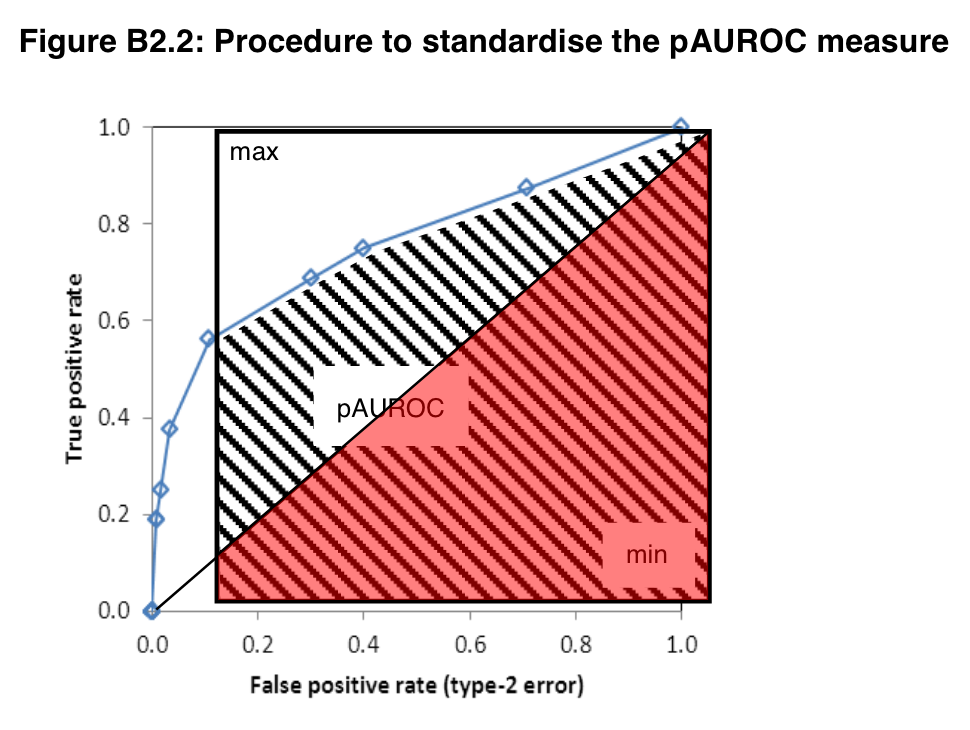
\includegraphics[width=0.7\linewidth]{../metadata/pAUC} \end{center}

\begin{align}
psAUROC = \frac{1}{2}\left[ 1+ \frac{pAUROC - min}{max - min}\right]
\end{align}

\hypertarget{model-selection-and-averaging}{%
\section{Model selection and averaging}\label{model-selection-and-averaging}}

\hypertarget{variable-selection}{%
\subsection{Variable selection}\label{variable-selection}}

\hypertarget{comparing-performance-of-individual-credit-gaps}{%
\subsubsection{Comparing performance of individual credit gaps}\label{comparing-performance-of-individual-credit-gaps}}

Using partial area under the curve (psAUC) values

\hypertarget{test-for-gaps-combination-performance}{%
\subsubsection{Test for gaps combination performance}\label{test-for-gaps-combination-performance}}

Using Markov Chain Monte Carlo Model Comparison (\(MC^3\)) developed by Madigan and York (1995). The method assigns posterior probability for different credit gaps being selected in most likely models/combinations. Babecky (2014) used this \(MC^3\) method to identify potential variables in EWI models.

\begin{align*}
Model_k :  pre.crisis_{ti} \sim \sum\nolimits_j \beta_j * credit.gap_{tij}
\end{align*}

\hypertarget{variable-selection-1}{%
\subsubsection{Variable selection}\label{variable-selection-1}}

We selected 29 credit gap measurements based on these 2 criteria.

\hypertarget{variable-selection-top-23-gaps-ranked-by-psauc}{%
\subsection{Variable selection (top 23 gaps ranked by psAUC)}\label{variable-selection-top-23-gaps-ranked-by-psauc}}

\begin{table}[H]
\centering
\resizebox{\linewidth}{!}{
\begin{tabular}[t]{lrrr>{}rrrrr}
\toprule
Cycles & BIC & AIC & AUC & psAUC & c.Threshold & Type.I & Type.II & Policy.Loss.Function\\
\midrule
null & 0.0000 & 0.0000 & 0.5000 & \textbf{0.5000} & NA & 1.0000 & 0.0000 & 1.0000\\
c.bn6.r20 & -108.0679 & -114.4506 & 0.7048 & \textbf{0.6379} & 0.6581 & 0.3962 & 0.3019 & 0.2481\\
c.hamilton28.panel & -149.8518 & -156.2346 & 0.7107 & \textbf{0.6359} & 9.7674 & 0.3912 & 0.3066 & 0.2470\\
c.hamilton13.panelr20 & -150.2442 & -156.6269 & 0.7036 & \textbf{0.6333} & 5.9895 & 0.4261 & 0.2547 & 0.2464\\
c.hamilton24.panel & -134.4093 & -140.7920 & 0.6991 & \textbf{0.6322} & 7.1794 & 0.4383 & 0.2689 & 0.2644\\
\addlinespace
c.hamilton20.panelr20 & -151.5617 & -157.9445 & 0.7048 & \textbf{0.6313} & 7.9350 & 0.4321 & 0.3066 & 0.2807\\
c.ma & -120.8108 & -127.1936 & 0.6922 & \textbf{0.6313} & 5.7813 & 0.3989 & 0.3160 & 0.2590\\
c.hamilton20.panelr15 & -135.3713 & -141.7540 & 0.6985 & \textbf{0.6312} & 7.5244 & 0.4616 & 0.2689 & 0.2854\\
c.hamilton13.panelr15 & -126.2968 & -132.6796 & 0.6924 & \textbf{0.6311} & 6.5289 & 0.4297 & 0.2830 & 0.2647\\
c.hamilton28.panelr20 & -164.6015 & -170.9842 & 0.7158 & \textbf{0.6302} & 10.8558 & 0.3948 & 0.2925 & 0.2414\\
\addlinespace
c.hamilton24.panelr20 & -155.8638 & -162.2466 & 0.7096 & \textbf{0.6301} & 9.1672 & 0.4251 & 0.2830 & 0.2608\\
c.hamilton24.panelr15 & -143.2235 & -149.6062 & 0.7033 & \textbf{0.6299} & 10.4963 & 0.3984 & 0.3160 & 0.2586\\
c.hamilton20.panel & -126.8625 & -133.2452 & 0.6907 & \textbf{0.6288} & 5.6212 & 0.4686 & 0.2830 & 0.2997\\
c.hamilton28.panelr15 & -154.4533 & -160.8361 & 0.7091 & \textbf{0.6270} & 11.5510 & 0.3854 & 0.2972 & 0.2369\\
c.hamilton13.panel & -133.9347 & -140.3175 & 0.6922 & \textbf{0.6250} & 4.9769 & 0.4285 & 0.2877 & 0.2664\\
\addlinespace
c.bn2.r20 & -109.3128 & -115.6955 & 0.6963 & \textbf{0.6218} & 0.2776 & 0.4080 & 0.3255 & 0.2724\\
c.linear & -135.4069 & -141.7896 & 0.6879 & \textbf{0.6204} & 3.9989 & 0.4616 & 0.2925 & 0.2986\\
c.bn2 & -135.9914 & -142.3741 & 0.6842 & \textbf{0.6165} & 0.1864 & 0.4530 & 0.3113 & 0.3021\\
c.bn6 & -132.7915 & -139.1742 & 0.6835 & \textbf{0.6113} & 0.4710 & 0.4371 & 0.2830 & 0.2712\\
c.bn6.r15 & -54.9953 & -61.3781 & 0.6756 & \textbf{0.6070} & 0.5680 & 0.4179 & 0.3255 & 0.2806\\
\addlinespace
c.bn2.r15 & -83.9469 & -90.3297 & 0.6749 & \textbf{0.6047} & 0.1349 & 0.4761 & 0.3302 & 0.3357\\
c.poly4.r20 & 3.5738 & -2.8090 & 0.5772 & \textbf{0.6011} & 0.1651 & 0.4980 & 0.3302 & 0.3570\\
BIS Basel gap & -121.5910 & -127.9738 & 0.6733 & \textbf{0.5960} & 3.0578 & 0.4441 & 0.3255 & 0.3032\\
c.bn4 & -169.1186 & -175.5014 & 0.6892 & \textbf{0.5943} & 1.2840 & 0.3837 & 0.3255 & 0.2532\\
c.bn4.r15 & -89.6147 & -95.9975 & 0.6669 & \textbf{0.5929} & 0.4435 & 0.4792 & 0.2925 & 0.3152\\
\addlinespace
c.bn5.r20 & -99.7674 & -106.1501 & 0.6744 & \textbf{0.5928} & 0.5016 & 0.4234 & 0.3302 & 0.2883\\
\bottomrule
\end{tabular}}
\end{table}

\hypertarget{variable-selection-mc3}{%
\subsection{Variable Selection (MC3)}\label{variable-selection-mc3}}

\tiny
\begin{table}[H]
\centering
\begin{tabular}[t]{lllr}
\toprule
Variable & Pr(B!=0) & Variable & Pr(B!=0)\\
\midrule
Intercept & 1 & c.bn2 & 0.3721\\
c.hamilton28\_panel & 0.999968 & c.bn3\_r10 & 0.2478\\
c.bn7\_r15 & 0.93097125 & c.hp400k & 0.2309\\
c.poly3 & 0.915792 & c.hamilton24\_r20 & 0.2175\\
c.hamilton13\_panel & 0.733247 & c.hamilton13\_r20 & 0.1958\\
\addlinespace
c.hamilton13\_r10 & 0.70601225 & c.bn2\_r10 & 0.1916\\
c.hamilton28 & 0.65141375 & c.stm & 0.1894\\
c.hamilton13 & 0.6438865 & c.hamilton28\_r20 & 0.1799\\
c.bn3\_r15 & 0.514728 & c.hp\_r20 & 0.1794\\
c.hp3k & 0.4888055 & c.hp & 0.1761\\
\addlinespace
c.hp3k\_r20 & 0.4887615 & c.bn8\_r20 & 0.1561\\
c.poly6 & 0.39826475 & c.linear\_r20 & 0.1526\\
 &  & c.hp221k & 0.1440\\
\bottomrule
\end{tabular}
\end{table}
\normalsize

\hypertarget{model-averaging}{%
\section{Model Averaging}\label{model-averaging}}

\hypertarget{model-averaging-1}{%
\section{Model averaging}\label{model-averaging-1}}

\hypertarget{bayesian-model-averging}{%
\subsection{Bayesian Model Averging}\label{bayesian-model-averging}}

The Bayesian Model Average method is formalized in Raftery (1995) to account for model uncertainty.

\hypertarget{model-posterior-probability}{%
\subsubsection{Model posterior probability}\label{model-posterior-probability}}

equation (33): Model k posterior probability (weight):
\begin{align}
  P(M_k|D) = \frac{P(D|M_k)P(M_k)}{\sum\nolimits_{l=1}^K P(D|M_l)P(M_l)} 
  \approx \frac{exp(-\frac{1}{2}BIC_k)}{\sum\nolimits_{l=1}^K exp(-\frac{1}{2}BIC_l)}
\end{align}

\begin{itemize}
\item
  Where \(P(M_k)\) is model prior probability and can be ignored if all models are assumed equal prior weights.
\item
  \(P(D|M_k)\) is marginal likehood. And \(P(D|M_k) \propto exp(-\frac{1}{2}BIC_k)\)
\item
  In which \(BIC_k = 2log (Bayesfactor_{sk}) = \chi^2_{sk} - df_klog(n)\). s indicates the saturated model.
\end{itemize}

\hypertarget{model-posterior-probability-1}{%
\subsection{Model posterior probability}\label{model-posterior-probability-1}}

\begin{itemize}
\tightlist
\item
  \(BIC_k = 2log (Bayesfactor_{sk}) = \chi^2_{sk} - df_klog(n)\)
\item
  \(\chi^2_{sk}\) is the deviance of model K from the the saturated model

  \begin{itemize}
  \tightlist
  \item
    \(\chi^2_{sk} = 2(ll(Ms) - ll(Mk))\)
  \item
    \(ll(Mk)\) is the log-likelihood of model Mk given data D
  \end{itemize}
\end{itemize}

\hypertarget{alternate-deviance-measurement}{%
\subsubsection{Alternate deviance measurement}\label{alternate-deviance-measurement}}

We propose using psAUC instead of log-likelihood in the measurement of deviance. Hence, an alternative BIC value can be estimated at:

\begin{align}
BIC_{alt,k} &= 2log (Bayesfactor_{alt,sk}) \\
&= 2(1000*(psAUC_s-psAUC_k)) - df_klog(n)
\end{align}
- We scaled the psAUC value by 1000 since \(0<psAUC<1\). Also, by design, \(psAUC_s=1\).

\hypertarget{posterior-distribution-of-coefficients-of-interest}{%
\subsection{Posterior distribution of coefficients of interest:}\label{posterior-distribution-of-coefficients-of-interest}}

\(\beta_j\) is the coefficient of credit gap j (\(c_j\)) in a logistic regression model k against pre-crisis indicator. When considering a particular \(\beta_1\) :

\begin{align*}
p(\beta_1|D, \beta_1\ne 0) = \sum\nolimits_{A_1} p(\beta_1|D,M_k)p'(M_k|D)
\end{align*}

\begin{itemize}
\tightlist
\item
  where \(p'(M_k|D)=p(M_k|D)/ pr[\beta_1 \ne 0|D]\)
\item
  and \(pr[\beta_1 \ne 0|D] = \sum\limits_{A_1} p(M_k|D)\)

  \begin{itemize}
  \tightlist
  \item
    this is the probability that \(\beta_1\) is in the averaged model
  \item
    \(A_1= \{M_k: k=1,...,K; \beta_1 \ne 0\}\), is the set of models that includes \(\beta_1\)
  \end{itemize}
\end{itemize}

\hypertarget{approximation-of-bayesian-point-estimate}{%
\subsection{Approximation of Bayesian point estimate:}\label{approximation-of-bayesian-point-estimate}}

\begin{align}
\hat{\beta}_1 = E[\beta_1|D, \beta_1\ne 0] = \sum\limits_{A_1} \hat{\beta}_1(k)p'(M_k|D)
\end{align}

\(SD^2[\beta_1|D, \beta_1\ne 0] =[\sum\limits_{A_1}[se_1^2(k)+]+\hat{\beta_1}(k)]p'(M_k|D) - E[\beta_1|D, \beta_1\ne 0]^2\)

\begin{itemize}
\tightlist
\item
  Where \(\hat{\beta}_1(k)\) and \(se_1^2(k)\) are respectively the MLE and standard error of \(\beta_1\) under the model \(M_k\). (Leamer 1978, p.118; Raftery 1993a)
\end{itemize}

\hypertarget{weighted-credit-gap-creation}{%
\section{Weighted credit gap creation}\label{weighted-credit-gap-creation}}

\hypertarget{weighted-averaged-credit-gap---motivation}{%
\subsection{Weighted averaged credit gap - motivation}\label{weighted-averaged-credit-gap---motivation}}

GLM binomial estimation:
\begin{align*}
\widehat{pre.crisis}_{ti} = \widehat{probability}_{ti} = \frac {1}{1+exp(-(a+\sum\nolimits_j \hat{\beta}_j c_{tij}))}
\end{align*}

\begin{itemize}
\tightlist
\item
  With \(\hat{\beta}_j\) = \(E[\beta_j|D, \beta_j\ne 0] = \sum\limits_{A_j} \hat{\beta}_j(k)p'(M_k|D)\)
\end{itemize}

\(\Rightarrow\) We propose a single weighted credit gap \(\hat{c}_{ti}\) that satisfies:
\begin{align*}
\frac {1}{1+exp(-(a+\hat{\beta} \hat{c}_{ti}))}= \frac {1}{1+exp(-(a+\sum\nolimits_j \hat{\beta}_j c_{tij}))} \\
\end{align*}
OR
\begin{align}
\sum\limits_j \hat{\beta}_j c_{tij} = \hat{\beta} \hat{c}_{ti}
\end{align}

\hypertarget{weighted-averaged-credit-gap---creation}{%
\subsection{Weighted averaged credit gap - creation}\label{weighted-averaged-credit-gap---creation}}

\begin{align*}
\sum\limits_j \hat{\beta}_j c_{tij} = \hat{\beta} \hat{c}_{ti}
\end{align*}

We then propose \(\hat{\beta} = \sum\nolimits_j \hat{\beta}_j\)

Therefore,

\begin{align}
\hat{c}_{ti} = \frac{\sum\nolimits_j (\hat{\beta}_j c_{tij})}{\sum\nolimits_j\hat{\beta}_j} = \sum\nolimits_j w_j c_{tij}
\end{align}

The weight of each candidate credit gap j is \(w_j = \frac{\hat{\beta}_j}{\sum\nolimits_j\hat{\beta}_j}\)

\hypertarget{one-sided-crisis-weighted-averaged-credit-gap}{%
\subsection{One-sided crisis weighted averaged credit gap}\label{one-sided-crisis-weighted-averaged-credit-gap}}

\begin{itemize}
\item
  The weight of each candidate credit gap j is \(w_j = \frac{\hat{\beta}_j}{\sum\nolimits_j\hat{\beta}_j}\)
\item
  We save the weights \(w_j\) at every incremental period \(t\) of available data to create a one-sided weight vector \(w_{tj}\).
\end{itemize}

\(\Rightarrow\) To create one-sided crisis weighted averaged credit gap for each country \(i\) (\(\hat{c}_{ti}\)), we compute:
\begin{align}
\hat{c}_{ti,one-sided} = \sum\nolimits_{j} w_{tj} * c_{tij}
\end{align}

\hypertarget{weights-stacked-graph}{%
\subsection{Weights stacked graph}\label{weights-stacked-graph}}

Weights are restricted to be positive to ensure stability

\begin{center}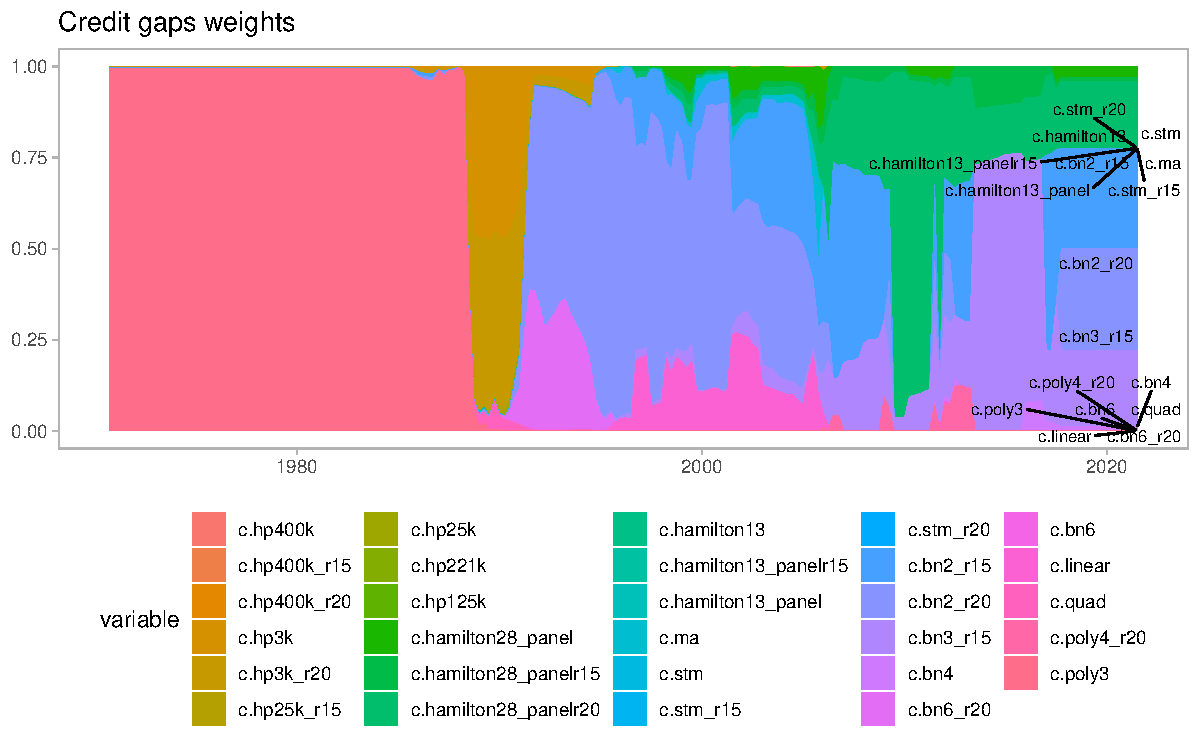
\includegraphics[width=1\linewidth]{../Data/Output/Graphs/Weights_stack} \end{center}

\hypertarget{weights-series-graph}{%
\subsection{Weights series graph}\label{weights-series-graph}}

\begin{center}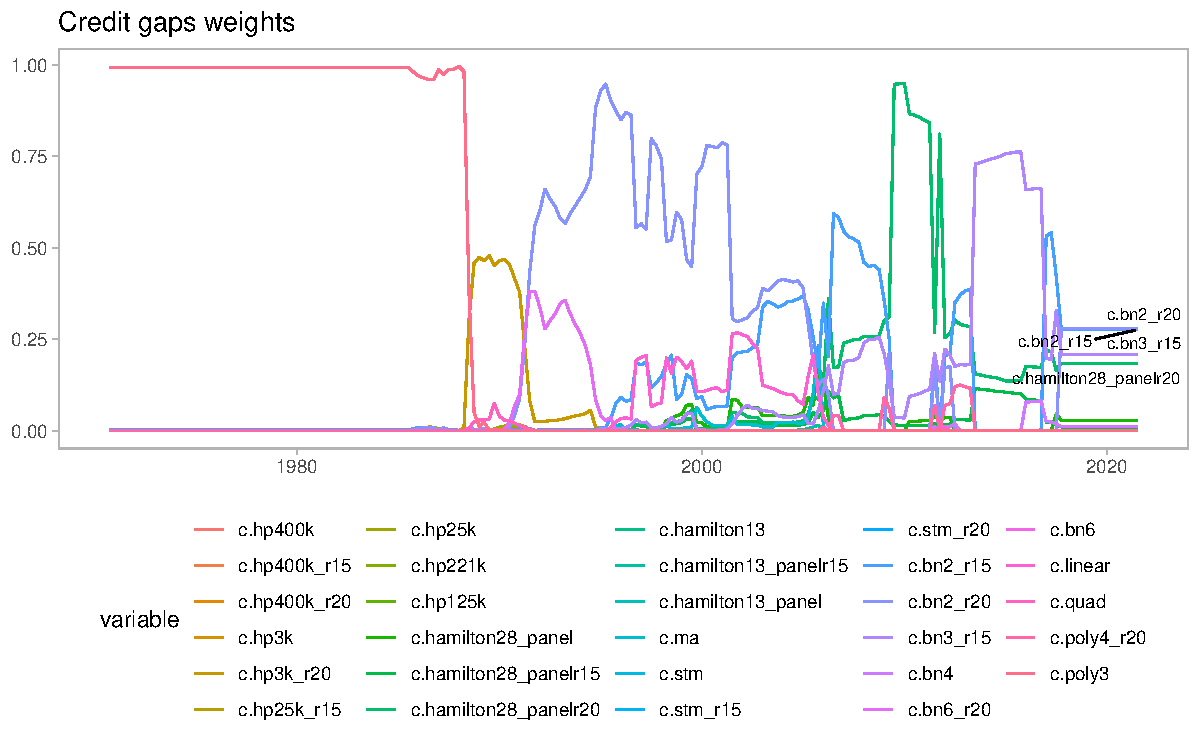
\includegraphics[width=1\linewidth]{../Data/Output/Graphs/Weights_series} \end{center}

\hypertarget{empirical-results}{%
\section{EMPIRICAL RESULTS}\label{empirical-results}}

\hypertarget{empirical-results-1}{%
\section{Empirical Results}\label{empirical-results-1}}

\hypertarget{comparing-performance-of-weighted-gap---full-sample}{%
\subsection{Comparing performance of weighted gap - Full Sample}\label{comparing-performance-of-weighted-gap---full-sample}}

\begin{table}[H]
\centering
\resizebox{\linewidth}{!}{
\begin{tabular}[t]{lrrr>{}rrrrr}
\toprule
Cycles & BIC & AIC & AUC & psAUC & c.Threshold & Type.I & Type.II & Policy.Loss.Function\\
\midrule
null & 0.0000 & 0.0000 & 0.5000 & \textbf{0.5000} & NA & 1.0000 & 0.0000 & 1.0000\\
\textbf{1.sided weighted.cycle} & \textbf{-127.5308} & \textbf{-133.9135} & \textbf{0.7182} & \textbf{\textbf{0.6454}} & \textbf{2.8892} & \textbf{0.3532} & \textbf{0.3255} & \textbf{0.2307}\\
c.bn6.r20 & -108.0679 & -114.4506 & 0.7048 & \textbf{0.6379} & 0.6581 & 0.3962 & 0.3019 & 0.2481\\
c.hamilton28.panel & -149.8518 & -156.2346 & 0.7107 & \textbf{0.6359} & 9.7674 & 0.3912 & 0.3066 & 0.2470\\
c.ma & -120.8108 & -127.1936 & 0.6922 & \textbf{0.6313} & 5.7813 & 0.3989 & 0.3160 & 0.2590\\
\addlinespace
c.hamilton13.panelr15 & -126.2968 & -132.6796 & 0.6924 & \textbf{0.6311} & 6.5289 & 0.4297 & 0.2830 & 0.2647\\
c.hamilton28.panelr20 & -164.6015 & -170.9842 & 0.7158 & \textbf{0.6302} & 10.8558 & 0.3948 & 0.2925 & 0.2414\\
c.hamilton28.panelr15 & -154.4533 & -160.8361 & 0.7091 & \textbf{0.6270} & 11.5510 & 0.3854 & 0.2972 & 0.2369\\
c.hamilton13.panel & -133.9347 & -140.3175 & 0.6922 & \textbf{0.6250} & 4.9769 & 0.4285 & 0.2877 & 0.2664\\
c.bn2.r20 & -109.3128 & -115.6955 & 0.6963 & \textbf{0.6218} & 0.2776 & 0.4080 & 0.3255 & 0.2724\\
\addlinespace
c.linear & -135.4069 & -141.7896 & 0.6879 & \textbf{0.6204} & 3.9989 & 0.4616 & 0.2925 & 0.2986\\
c.bn6 & -132.7915 & -139.1742 & 0.6835 & \textbf{0.6113} & 0.4710 & 0.4371 & 0.2830 & 0.2712\\
c.bn2.r15 & -83.9469 & -90.3297 & 0.6749 & \textbf{0.6047} & 0.1349 & 0.4761 & 0.3302 & 0.3357\\
c.poly4.r20 & 3.5738 & -2.8090 & 0.5772 & \textbf{0.6011} & 0.1651 & 0.4980 & 0.3302 & 0.3570\\
\textbf{BIS Basel gap} & \textbf{-121.5910} & \textbf{-127.9738} & \textbf{0.6733} & \textbf{\textbf{0.5960}} & \textbf{3.0578} & \textbf{0.4441} & \textbf{0.3255} & \textbf{0.3032}\\
\addlinespace
c.bn4 & -169.1186 & -175.5014 & 0.6892 & \textbf{0.5943} & 1.2840 & 0.3837 & 0.3255 & 0.2532\\
c.stm.r15 & -79.5531 & -85.9358 & 0.6575 & \textbf{0.5924} & 2.0027 & 0.4778 & 0.3160 & 0.3281\\
c.hp125k & -92.2897 & -98.6725 & 0.6562 & \textbf{0.5924} & 2.5216 & 0.4547 & 0.3302 & 0.3158\\
c.hp221k & -106.8842 & -113.2670 & 0.6656 & \textbf{0.5921} & 2.6641 & 0.4561 & 0.3160 & 0.3079\\
c.hp400k.r15 & -67.1228 & -73.5055 & 0.6472 & \textbf{0.5912} & 2.6223 & 0.4592 & 0.3255 & 0.3168\\
\addlinespace
c.stm & -89.2228 & -95.6055 & 0.6523 & \textbf{0.5903} & 2.2064 & 0.4684 & 0.3302 & 0.3284\\
c.bn3.r15 & -144.4817 & -150.8645 & 0.6687 & \textbf{0.5882} & 0.1862 & 0.4780 & 0.3302 & 0.3375\\
c.hp400k.r20 & -88.8450 & -95.2277 & 0.6545 & \textbf{0.5871} & 2.8130 & 0.4494 & 0.3302 & 0.3110\\
c.stm.r20 & -87.2179 & -93.6006 & 0.6482 & \textbf{0.5859} & 1.9362 & 0.4826 & 0.3302 & 0.3419\\
c.hp25k.r15 & -55.8805 & -62.2632 & 0.6275 & \textbf{0.5812} & 1.1403 & 0.5032 & 0.3066 & 0.3473\\
\addlinespace
c.hp25k & -56.0388 & -62.4215 & 0.6274 & \textbf{0.5782} & 1.2839 & 0.4970 & 0.3160 & 0.3469\\
c.hamilton13 & -23.7688 & -30.1516 & 0.6075 & \textbf{0.5782} & 1.6938 & 0.5006 & 0.3160 & 0.3505\\
c.quad & -85.1640 & -91.5468 & 0.6622 & \textbf{0.5774} & 0.2765 & 0.5162 & 0.3160 & 0.3664\\
c.poly3 & 5.5099 & -0.8728 & 0.5551 & \textbf{0.5597} & -0.5367 & 0.5860 & 0.2689 & 0.4156\\
c.hp3k & -24.5546 & -30.9374 & 0.5979 & \textbf{0.5572} & -0.0472 & 0.5706 & 0.3255 & 0.4315\\
\addlinespace
c.hp3k.r20 & -24.5252 & -30.9080 & 0.5978 & \textbf{0.5571} & -0.0420 & 0.5701 & 0.3255 & 0.4309\\
\bottomrule
\end{tabular}}
\end{table}

\hypertarget{comparing-performance-of-weighted-gap-as-an-ewi---ae}{%
\subsection{Comparing performance of weighted gap as an EWI - AE}\label{comparing-performance-of-weighted-gap-as-an-ewi---ae}}

\begin{table}[H]
\centering
\resizebox{\linewidth}{!}{
\begin{tabular}[t]{lrrr>{}rrrrr}
\toprule
Cycles & BIC & AIC & AUC & psAUC & c.Threshold & Type.I & Type.II & Policy.Loss.Function\\
\midrule
null & 0.0000 & 0.0000 & 0.5000 & \textbf{0.5000} & NA & 1.0000 & 0.0000 & 1.0000\\
\textbf{1.sided weighted.cycle} & \textbf{-128.8749} & \textbf{-134.9430} & \textbf{0.7545} & \textbf{\textbf{0.6889}} & \textbf{3.5486} & \textbf{0.3177} & \textbf{0.2841} & \textbf{0.1817}\\
c.hamilton13.panelr15 & -116.9260 & -122.9941 & 0.7282 & \textbf{0.6846} & 8.8000 & 0.3469 & 0.3011 & 0.2110\\
c.hamilton28.panelr15 & -141.5772 & -147.6453 & 0.7491 & \textbf{0.6825} & 11.5510 & 0.3834 & 0.2216 & 0.1961\\
c.hamilton28.panelr20 & -147.4322 & -153.5003 & 0.7514 & \textbf{0.6811} & 13.1072 & 0.3489 & 0.2898 & 0.2057\\
\addlinespace
c.bn6.r20 & -90.1022 & -96.1703 & 0.7338 & \textbf{0.6751} & 0.6581 & 0.4126 & 0.2273 & 0.2219\\
c.hamilton28.panel & -129.1730 & -135.2411 & 0.7382 & \textbf{0.6740} & 9.7674 & 0.3977 & 0.2386 & 0.2151\\
c.hamilton13.panel & -122.0054 & -128.0735 & 0.7208 & \textbf{0.6684} & 7.2247 & 0.3509 & 0.3239 & 0.2280\\
c.ma & -97.4868 & -103.5549 & 0.7133 & \textbf{0.6677} & 6.0375 & 0.4073 & 0.2727 & 0.2403\\
c.bn6 & -104.1404 & -110.2085 & 0.7042 & \textbf{0.6426} & 0.8256 & 0.4040 & 0.2955 & 0.2505\\
\addlinespace
c.hp125k & -92.8331 & -98.9012 & 0.6977 & \textbf{0.6397} & 3.6972 & 0.3788 & 0.3239 & 0.2484\\
\textbf{BIS Basel gap} & \textbf{-113.9826} & \textbf{-120.0507} & \textbf{0.7124} & \textbf{\textbf{0.6390}} & \textbf{3.9706} & \textbf{0.3847} & \textbf{0.3011} & \textbf{0.2387}\\
c.hp221k & -104.1190 & -110.1871 & 0.7070 & \textbf{0.6388} & 3.8869 & 0.3755 & 0.3011 & 0.2317\\
c.stm.r15 & -86.6063 & -92.6744 & 0.6989 & \textbf{0.6382} & 4.0784 & 0.3486 & 0.3295 & 0.2301\\
c.stm & -89.9073 & -95.9754 & 0.6929 & \textbf{0.6357} & 3.3071 & 0.3924 & 0.3295 & 0.2626\\
\addlinespace
c.hp400k.r15 & -73.5902 & -79.6582 & 0.6869 & \textbf{0.6357} & 4.2355 & 0.3496 & 0.3125 & 0.2199\\
c.linear & -111.9570 & -118.0251 & 0.7069 & \textbf{0.6356} & 3.9964 & 0.4620 & 0.2443 & 0.2732\\
c.hp400k.r20 & -93.8576 & -99.9257 & 0.6991 & \textbf{0.6340} & 4.3393 & 0.3622 & 0.3295 & 0.2398\\
c.bn2.r20 & -84.0800 & -90.1481 & 0.6955 & \textbf{0.6297} & 0.2773 & 0.4216 & 0.3182 & 0.2790\\
c.stm.r20 & -87.6992 & -93.7673 & 0.6879 & \textbf{0.6282} & 3.1055 & 0.4073 & 0.3239 & 0.2708\\
\addlinespace
c.bn4 & -119.0600 & -125.1280 & 0.7038 & \textbf{0.6272} & 1.8875 & 0.3575 & 0.3295 & 0.2364\\
c.hp25k.r15 & -54.6351 & -60.7032 & 0.6561 & \textbf{0.6138} & 1.6927 & 0.4547 & 0.2784 & 0.2843\\
c.hp25k & -55.5895 & -61.6576 & 0.6569 & \textbf{0.6117} & 1.7847 & 0.4458 & 0.2898 & 0.2827\\
c.poly4.r20 & 2.3864 & -3.6817 & 0.5901 & \textbf{0.6113} & 0.7143 & 0.4494 & 0.3239 & 0.3069\\
c.quad & -88.1553 & -94.2234 & 0.6998 & \textbf{0.6099} & 2.4569 & 0.4017 & 0.3295 & 0.2699\\
\addlinespace
c.bn2.r15 & -62.5255 & -68.5936 & 0.6683 & \textbf{0.6070} & 0.0956 & 0.5075 & 0.3011 & 0.3482\\
c.hamilton13 & -29.9493 & -36.0174 & 0.6334 & \textbf{0.6028} & 3.3153 & 0.4398 & 0.3239 & 0.2983\\
c.bn3.r15 & -93.9600 & -100.0281 & 0.6534 & \textbf{0.5836} & 0.1563 & 0.4896 & 0.3239 & 0.3445\\
c.hp3k & -20.4943 & -26.5624 & 0.6092 & \textbf{0.5725} & 0.1378 & 0.5446 & 0.3068 & 0.3907\\
c.hp3k.r20 & -20.4682 & -26.5363 & 0.6091 & \textbf{0.5724} & 0.1378 & 0.5446 & 0.3068 & 0.3907\\
\addlinespace
c.poly3 & -2.3248 & -8.3929 & 0.5905 & \textbf{0.5723} & 0.2767 & 0.5317 & 0.3295 & 0.3913\\
\bottomrule
\end{tabular}}
\end{table}

\hypertarget{comparing-performance-of-weighted-gap-as-an-ewi---eme}{%
\subsection{Comparing performance of weighted gap as an EWI - EME}\label{comparing-performance-of-weighted-gap-as-an-ewi---eme}}

\begin{table}[H]
\centering
\resizebox{\linewidth}{!}{
\begin{tabular}[t]{lrrr>{}rrrrr}
\toprule
Cycles & BIC & AIC & AUC & psAUC & c.Threshold & Type.I & Type.II & Policy.Loss.Function\\
\midrule
null & 0.0000 & 0.0000 & 0.5000 & \textbf{0.5000} & NA & 1.0000 & 0.0000 & 1.0000\\
c.bn3.r15 & -46.2774 & -51.3507 & 0.7365 & \textbf{0.6308} & 0.6244 & 0.3059 & 0.3333 & 0.2047\\
c.poly3 & 5.3862 & 0.3129 & 0.5737 & \textbf{0.6046} & 1.8089 & 0.5280 & 0.3056 & 0.3721\\
c.bn2.r15 & -13.2062 & -18.2795 & 0.6879 & \textbf{0.5879} & 0.2952 & 0.3566 & 0.3333 & 0.2383\\
c.poly4.r20 & 7.0732 & 1.9999 & 0.5040 & \textbf{0.5816} & -0.9609 & 0.5962 & 0.3333 & 0.4665\\
\addlinespace
\textbf{1.sided weighted.cycle} & \textbf{6.2094} & \textbf{1.1361} & \textbf{0.5325} & \textbf{\textbf{0.5811}} & \textbf{-1.0639} & \textbf{0.6827} & \textbf{0.1111} & \textbf{0.4784}\\
c.linear & -9.3676 & -14.4409 & 0.5787 & \textbf{0.5774} & -0.9783 & 0.6294 & 0.2222 & 0.4455\\
c.bn2.r20 & -16.6411 & -21.7144 & 0.6760 & \textbf{0.5751} & 0.1470 & 0.4510 & 0.3056 & 0.2968\\
c.hamilton13 & 6.5749 & 1.5016 & 0.5468 & \textbf{0.5710} & 3.6354 & 0.6206 & 0.3056 & 0.4785\\
c.ma & -11.6401 & -16.7133 & 0.5572 & \textbf{0.5457} & -0.2250 & 0.7220 & 0.1667 & 0.5491\\
\addlinespace
c.hamilton28.panel & -7.8687 & -12.9420 & 0.5392 & \textbf{0.5384} & -1.7750 & 0.6958 & 0.2778 & 0.5613\\
c.quad & 6.1997 & 1.1264 & 0.4654 & \textbf{0.5334} & -6.4882 & 0.7456 & 0.1944 & 0.5938\\
c.hamilton13.panelr15 & -1.6660 & -6.7393 & 0.5087 & \textbf{0.5274} & -1.1064 & 0.7002 & 0.3333 & 0.6014\\
c.hp25k.r15 & 3.6420 & -1.4313 & 0.5018 & \textbf{0.5265} & -3.5672 & 0.7850 & 0.1111 & 0.6285\\
c.hp25k & 3.9466 & -1.1267 & 0.4975 & \textbf{0.5247} & -3.7339 & 0.7893 & 0.1111 & 0.6354\\
\addlinespace
c.hp3k & 3.3678 & -1.7054 & 0.5276 & \textbf{0.5235} & -1.1119 & 0.7019 & 0.3333 & 0.6038\\
c.hp3k.r20 & 3.3703 & -1.7030 & 0.5276 & \textbf{0.5235} & -1.1125 & 0.7028 & 0.3333 & 0.6050\\
c.hamilton13.panel & -1.6294 & -6.7027 & 0.5166 & \textbf{0.5222} & -2.9398 & 0.7500 & 0.2778 & 0.6397\\
\textbf{BIS Basel gap} & \textbf{-0.7015} & \textbf{-5.7748} & \textbf{0.4928} & \textbf{\textbf{0.5217}} & \textbf{-5.3969} & \textbf{0.7920} & \textbf{0.1389} & \textbf{0.6465}\\
c.hamilton28.panelr20 & -4.9986 & -10.0719 & 0.5123 & \textbf{0.5213} & -1.5578 & 0.6932 & 0.3333 & 0.5916\\
\addlinespace
c.hamilton28.panelr15 & -3.3914 & -8.4647 & 0.4987 & \textbf{0.5162} & -1.8326 & 0.7220 & 0.3333 & 0.6324\\
c.hp400k.r15 & 5.0603 & -0.0129 & 0.4777 & \textbf{0.5147} & -5.7358 & 0.8121 & 0.1111 & 0.6718\\
c.stm.r15 & 4.7567 & -0.3166 & 0.4780 & \textbf{0.5129} & -5.6472 & 0.8191 & 0.0833 & 0.6778\\
c.hp221k & 1.5902 & -3.4831 & 0.4787 & \textbf{0.5123} & -5.6416 & 0.8121 & 0.1111 & 0.6718\\
c.stm.r20 & 3.1397 & -1.9336 & 0.4768 & \textbf{0.5095} & -5.3727 & 0.8226 & 0.0833 & 0.6835\\
\addlinespace
c.hp125k & 3.0774 & -1.9958 & 0.4740 & \textbf{0.5094} & -5.8918 & 0.8226 & 0.0833 & 0.6835\\
c.stm & 3.1932 & -1.8801 & 0.4757 & \textbf{0.5087} & -5.5221 & 0.8260 & 0.0833 & 0.6893\\
c.hp400k.r20 & 4.1478 & -0.9255 & 0.4596 & \textbf{0.5081} & -6.2903 & 0.8182 & 0.1389 & 0.6887\\
c.bn4 & -42.1713 & -47.2446 & 0.5479 & \textbf{0.4984} & -0.5515 & 0.7509 & 0.2778 & 0.6410\\
c.bn6.r20 & -9.5340 & -14.6072 & 0.5296 & \textbf{0.4965} & -0.5188 & 0.7002 & 0.2778 & 0.5674\\
\addlinespace
c.bn6 & -19.2453 & -24.3186 & 0.5352 & \textbf{0.4911} & -0.5146 & 0.7220 & 0.2778 & 0.5985\\
\bottomrule
\end{tabular}}
\end{table}

\hypertarget{plot-weighted-gap-against-bis-gap}{%
\subsection{Plot weighted gap against BIS gap}\label{plot-weighted-gap-against-bis-gap}}

\begin{center}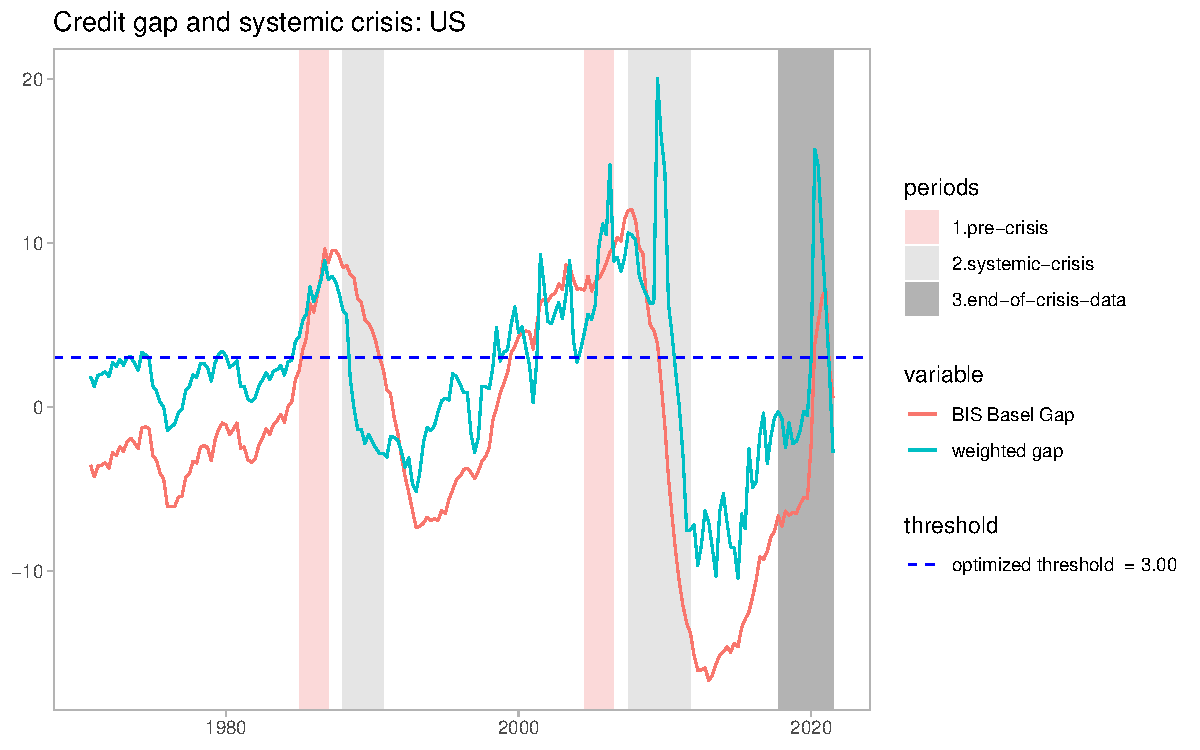
\includegraphics[width=1\linewidth]{../Data/Output/Graphs/Weighted_credit_gap_US} \end{center}

\hypertarget{plot-weighted-gap-against-bis-gap-1}{%
\subsection{Plot weighted gap against BIS gap}\label{plot-weighted-gap-against-bis-gap-1}}

\begin{center}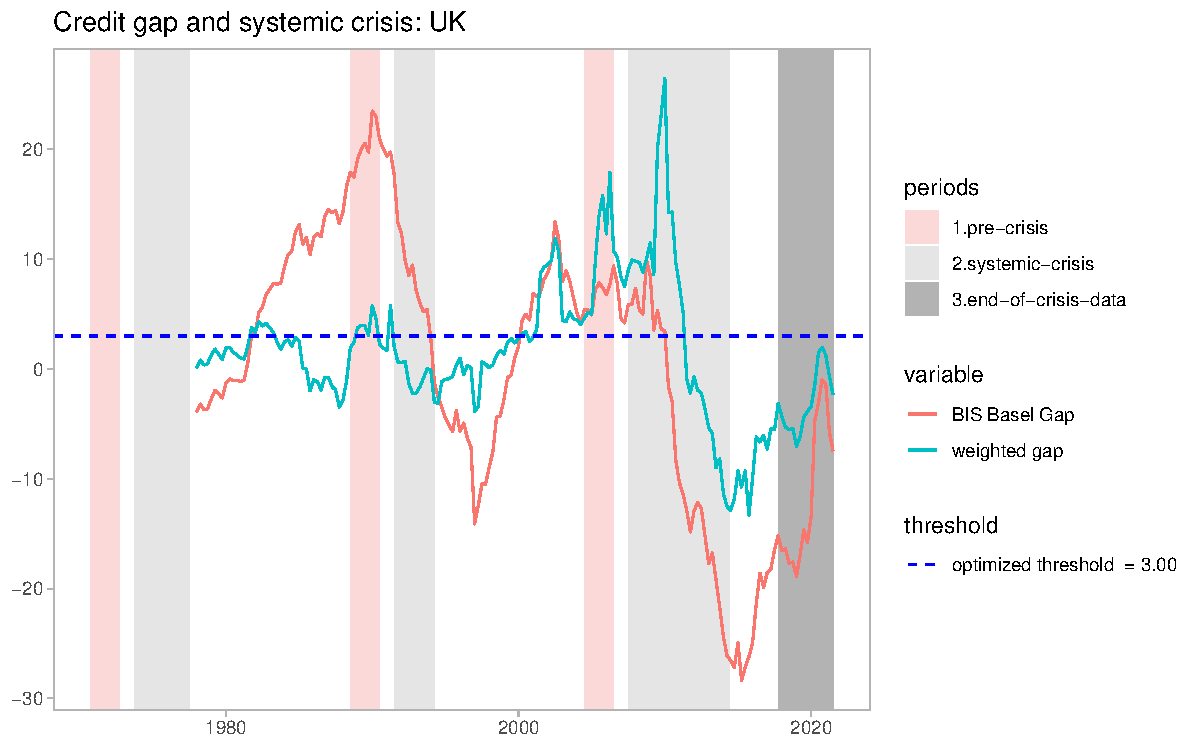
\includegraphics[width=1\linewidth]{../Data/Output/Graphs/Weighted_credit_gap_UK} \end{center}

\hypertarget{comparison-with-other-decomposition-methods}{%
\section{Comparison with other decomposition methods}\label{comparison-with-other-decomposition-methods}}

\hypertarget{conclusion}{%
\section{Conclusion}\label{conclusion}}

\hypertarget{appendix}{%
\section*{APPENDIX}\label{appendix}}
\addcontentsline{toc}{section}{APPENDIX}

\end{document}
